\documentclass[10pt,a4paper]{article}
\usepackage[margin=2.2cm]{geometry}
\usepackage{fontspec}
\usepackage{kotex}
\setmainfont{Apple SD Gothic Neo}
\setsansfont{Apple SD Gothic Neo}
\usepackage{amsmath,amssymb}
\usepackage{graphicx}
\usepackage{booktabs}
\usepackage{caption}
\usepackage[dvipsnames]{xcolor}
\usepackage[colorlinks=true,linkcolor=MidnightBlue,citecolor=MidnightBlue,
            urlcolor=MidnightBlue]{hyperref}
\usepackage{titlesec}
\titleformat{\section}{\large\bfseries}{\thesection}{0.6em}{}
\titleformat{\subsection}{\normalsize\bfseries}{\thesubsection}{0.5em}{}
\captionsetup{font=small,labelfont=bf}
\setlength{\parskip}{0.35em}
\setlength{\parindent}{0pt}

\usepackage{mdframed}
\newmdenv[linewidth=0.4pt,linecolor=gray!60,backgroundcolor=gray!5,
          innertopmargin=6pt,innerbottommargin=6pt,skipabove=8pt,skipbelow=8pt]{claimbox}
\newcommand{\claim}[2]{\begin{claimbox}\textbf{주장.} #1\par\smallskip
  \textcolor{gray!70}{\textbf{반증 조건.} #2}\end{claimbox}}

\title{\bfseries 판을 올린 첫 열\\[2pt]
\large 만화 세 열이 위약 여섯을 다 이겼다 --- 그래도 채택하지 않는다}
\author{월드모델 실험실 · 노트 778 $\sim$ 781}
\date{2026-08-07}
\begin{document}\maketitle

\section{한 줄}

논문 $154$ 가 \texttt{rawaxes.SPEC} 이 훑지 않은 세 도메인(만화 · 게임 · 도서)의
$11$열을 찾았다. 그 관례 그대로 만들고 --- \textbf{라벨을 한 번도 안 보고} ---
\textbf{노트 $348$ 의 순서로 도메인 하나씩} 쟀다.

\textbf{만화 세 열이 통과했다.} 신호 몫 $\mathbf{+0.0231}$ 이 \textbf{못박은 자
둘}($2 \times$뽑기SD $0.0200$ · 그 도메인 $2\sigma$ $0.0163$)\textbf{을 다 넘고},
\textbf{위약 여섯을 전부 이긴다}($6/6$). \textbf{판도 $0.4697 \to 0.4717$ 로
올랐다.}

\textbf{이 세션에서 판을 올린 첫 열이다. 그래도 채택하지 않는다} --- 규약
$12$(집안 $\geq 1$ · \textbf{집 밖 $\geq 2$}).

\section{만든 법 --- 라벨을 한 번도 안 봤다}

\texttt{rawaxes} 관례 그대로다: 범주형은 \textbf{집단 크기 순 $0{\sim}1$}($20$건 미만
마스크 $0$), 수치형은 \textbf{관측값만 \texttt{rankdata} 백분위}(동률을 행 순서로
깨지 않는다는 노트 $292$ 의 단언 포함).

\begin{center}
\begin{tabular}{llrl}
\toprule
도메인(학습행) & 열 & 값 가짓수 & \\
\midrule
\textbf{만화}($5{,}644$) & \texttt{mg\_format} · \texttt{mg\_adult} · \texttt{mg\_nauthor} & $3 \cdot 2 \cdot 9$ & \\
게임($259$) & \texttt{gm\_free} · \texttt{gm\_ndlc} · \texttt{gm\_nplat} & $2 \cdot 55 \cdot 3$ & \\
도서($80$) & \texttt{bk\_format} · \texttt{bk\_pages} · 폭 · 높이 · 무게 & $2 \cdot \ldots$ & $5$열 \\
\bottomrule
\end{tabular}
\end{center}

\textbf{배선 통과}: $11$열 전부 만들어지고 빠진 열 없음 · 행수가 판과 정확히
일치(만화 $5{,}905$ · 게임 $482$ · 도서 $243$) · 마스크 $0.99{\sim}1.00$ · 기준선
$0.4697$(노트 $737$ 과 일치).

\textbf{그리고 묶음으로 넣지 않았다} --- 논문 $154$ 가 되찾은 노트 $348$ 의 교훈이
그것이다(묶음 판 $-0.0027$ 대 갈라서 넷 $+0.0068$).

\begin{figure}[t]\centering
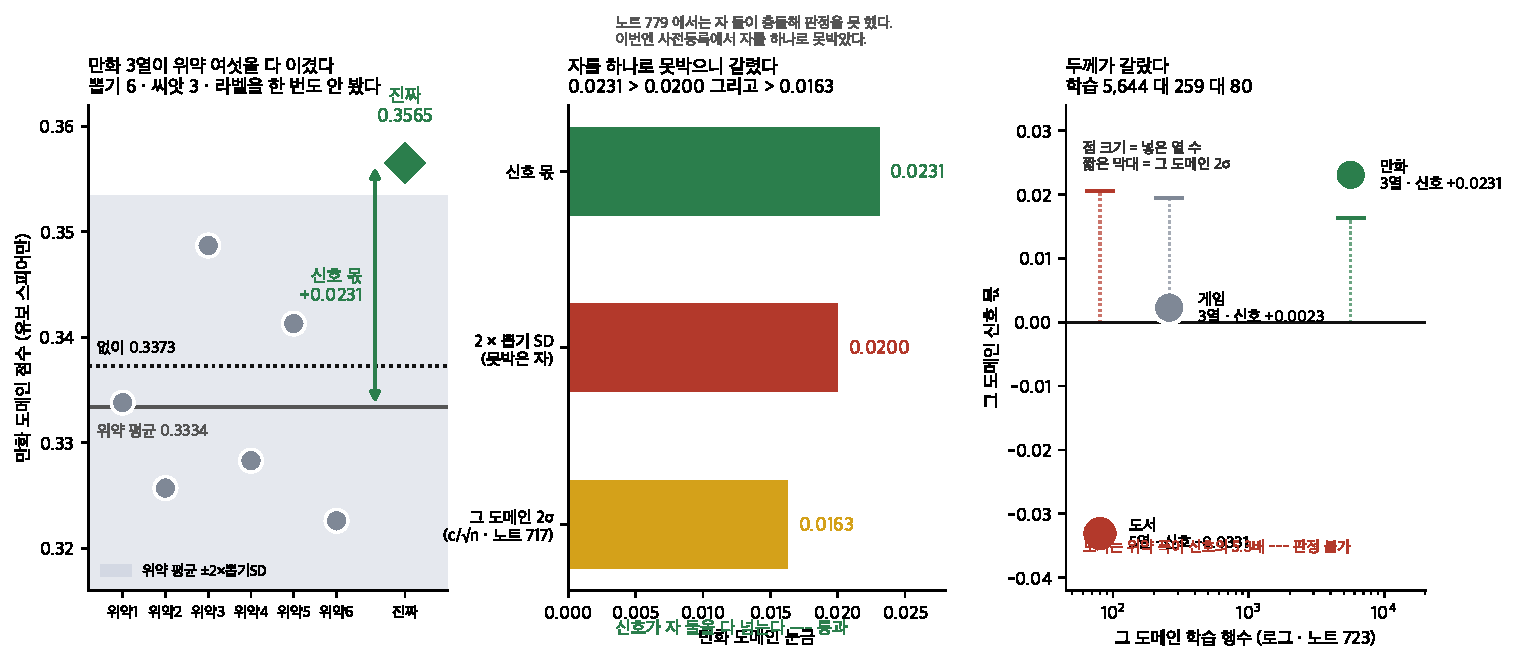
\includegraphics[width=0.99\textwidth]{figs/firstpass.pdf}
\caption{왼쪽: \textbf{만화 $3$열이 위약 여섯을 다 이겼다.} 가운데: \textbf{자를 하나로
못박으니 갈렸다.} 오른쪽: \textbf{두께가 갈랐다} --- 학습 $5{,}644$ 대 $259$ 대 $80$.}
\end{figure}

\section{만화 --- 통과}

\begin{center}
\begin{tabular}{lrl}
\toprule
없이(만화 점수) & $0.3373$ & \\
\textbf{진짜} & $\mathbf{0.3565}$ & \\
위약 뽑기 $6$ & $0.3338 \cdot 0.3257 \cdot 0.3487 \cdot 0.3283 \cdot 0.3413 \cdot 0.3226$ & 평균 $0.3334$ · SD $0.00999$ \\
\midrule
\textbf{신호 몫} & $\mathbf{+0.0231}$ & \\
$2 \times$뽑기SD (못박은 자) & $0.0200$ & \textbf{넘는다} \\
그 도메인 $2\sigma$ & $0.0163$ & \textbf{넘는다} \\
위약 전부보다 큼 & $6/6$ & 우연이면 $1/7$ \\
\midrule
판 & $0.4697 \to \mathbf{0.4717}$ & $+0.0020$ · 판 위약 평균 대비 $+0.0031$ \\
\bottomrule
\end{tabular}
\end{center}

\claim{\textbf{자를 하나로 못박은 것이 값을 했다.} 첫 판(뽑기 $3$)에서 신호 몫
$+0.0204$ 를 얻었는데 \textbf{내 사전등록 규칙이 모호해 판정을 못 했다} ---
\emph{``위약 전부보다 큰가(폭이 신호보다 크면 판정 안 함)''}에서 앞 조건은 참이고 뒤
조건은 위반이었다(폭 $0.0230 >$ 신호 $0.0204$). \textbf{그래서 다음 사전등록에서
$2 \times$뽑기SD 하나로 못박았고, 뽑기를 $6$ 으로 늘려 한 줄로 갈렸다.}}
{$2\times$SD 도 임의 선택이다 --- $3\times$SD($0.0300$)로 잡으면 통과하지 못한다.
\textbf{그 선택을 결과 보기 전에 적었다는 것이 이 판정의 근거이고, 다른 자로 읽으면
결론이 바뀔 수 있다는 뜻이다.} 그래서 \textbf{집 밖 둘}(규약 $12$)이 필요하다 ---
자의 선택이 아니라 \emph{다른 표본}이 판정하게 하는 것.}

\subsection*{🔴 그래도 채택하지 않는다}

노트 $133$(\emph{``첫 양성을 그냥 채택하지 않는다''})과 \textbf{규약 $12$}(집안
$\geq 1$ · \textbf{집 밖 $\geq 2$})를 따른다. 그 규약은 \textbf{실측 오탐률}로
세워졌다 --- 집 밖 $\geq 1$ 은 $33.8\%$, $\geq 2$ 는 $2.3\%$(노트 $715$).

\begin{center}
\textbf{집 밖 둘을 넘기 전에는 \texttt{rawaxes.SPEC} 과 \texttt{RAW\_KEEP} 을 안
고친다.}\\
다음: 앱($0.024$) · KR만화($0.025$) · CN만화($0.022$) 짝 채점.
\end{center}

\section{게임과 도서 --- 그리고 두께가 갈랐다}

\begin{center}
\begin{tabular}{lrrrl}
\toprule
도메인 & 학습행 & 신호 몫 & 그 $2\sigma$ & \\
\midrule
\textbf{만화} & $5{,}644$ & $\mathbf{+0.0231}$ & $0.0163$ & \textbf{통과} \\
게임 & $259$ & $+0.0023$ & $0.0195$ & 미달($2\sigma$ 의 $1/8$) \\
도서 & $80$ & $-0.0331$ & $0.0205$ & \textbf{판정 불가} \\
\bottomrule
\end{tabular}
\end{center}

\textbf{도서는 ``해롭다''가 아니라 ``못 가른다''다} --- 위약 셋이 $0.3146 \cdot
0.1689 \cdot 0.3440$ 으로 \textbf{폭이 $0.1751$} 이고 $|$신호 몫$|$($0.0331$)의
\textbf{$5.3$배}다. 사전등록 규칙의 괄호가 정확히 이 경우를 막았다.

\claim{\textbf{세 도메인의 차이가 ``열의 내용''보다 ``도메인의 두께''로 설명된다.}
학습행 $5{,}644 \cdot 259 \cdot 80$ 이고 결과가 통과 · 미달 · 판정불가다.
\textbf{도서의 물리 치수는 시간 게이트가 가장 깨끗했는데}(출간 시점 확정 · 인기와 함께
안 자란다) \textbf{$80$행에 $5$열을 넣어 그 이득을 볼 수 없었다} --- 노트 $641$ 의
얇은 도메인 비용($열당 0.02{\sim}0.025$)으로 $5$열이면 $0.10{\sim}0.125$ 이고 실측
$-0.1462$ 가 그 자리다.}
{두께가 아니라 \textbf{열의 내용}일 수도 있다 --- 만화의 세 열이 우연히 좋았을 수 있다.
\textbf{가르는 실험을 등록했다}: 게임 · 도서에 \textbf{$1$열만} 넣으면 얇은 도메인
비용이 $0.02{\sim}0.025$ 로 줄고, 그때도 못 넘으면 \textbf{두께가 아니라 내용}이다.}

\subsection*{내 예측이 가장 크게 틀린 곳}

사전등록에서 \emph{``도서가 가장 유망''}(신호 몫 $0.00 \sim 0.06$)이라 적었고
\textbf{$-0.0331$ 로 가장 나빴다.}

\claim{\textbf{나는 ``시간 게이트가 깨끗하다''를 ``신호가 있다''로 읽었다.} 물리
치수는 누출이 없지만 \textbf{얇은 도메인에 $5$열은 비싸다} --- \textbf{두 가드가 반대
방향으로 걸리는데 나는 하나만 봤다}(시간 게이트 통과 $\to$ 유망 / 얇은 도메인 열
예산 $\to$ 비쌈).}
{그렇다면 도서에 \textbf{가장 깨끗한 $1$열만} 넣어야 했다. \textbf{그것을 미결에
값으로 적었다} --- 다만 어느 $1$열을 고르나가 다시 선택이고, 결과를 보고 고르면
체리피킹이다. \textbf{사전에 고르는 규칙이 필요하고 그것을 아직 안 적었다.}}

\section{왜 만화였나 --- 안 쟀다}

만화는 \textbf{유보 $258$행이지만 학습 $5{,}644$행으로 판에서 가장 두껍다}(노트
$723$). 그리고 \textbf{도메인 전용 열이 하나도 없던 도메인}이다(논문 $154$) --- 즉
그 도메인 자료가 판에 거의 안 들어가 있었다.

\claim{\textbf{``두꺼운데 전용 열이 없던 도메인''이 가장 큰 이득을 낼 자리였다}는 것이
그럴듯한 설명이다. \textbf{그러나 안 쟀다} --- 열 하나씩 갈라 재면 어느 열이 냈나가
나오고, 그것이 다음 미결이다.}
{설명이 사후적이다 --- \textbf{나는 예측에서 만화를 $-0.02 \sim +0.02$ 로 적었고
$+0.0204$ 로 살짝 밖이었다.} 즉 \textbf{이 설명은 결과를 보고 만든 것}이고, 시험은
게임 · 도서에 $1$열을 넣는 실험이 한다.}

\end{document}
